\documentclass[paper-main.tex]{subfiles}


\begin{document}


 
% Tracking tones with the Viterbi algorithm
% explaination and successful application
% lean on the continuous gravitational waves angle
Continuous wave signals may wander slowly in frequency over time. 
%As also mentioned in Section~\ref{sec:introduction}, continuous wave searches often look for signals that wander slowly in frequency~\cite{ScoX1O2Viterbi:2019}. 
The audio analogue of this is a tone that wanders in frequency; a note that changes pitch. 
%Unlike the single tone described in Section~\ref{sec:single_tone}, finding the signal isn’t as simple as searching for a peak in the spectrum for the full timeseries data.%observing run.


The analysis techniques used here are inspired by those used to search for continuous waves from spinning neutron in LIGO and Virgo data~\cite{SuvorovaEtAl:2016,SuvorovaEtAl:2017}.
Continuous wave searches are performed on long datasets (months to years in duration). 
The frequency of gravitational-wave emission wanders significantly over the observation period. 

One method to search for a wandering signal is to split the data into several shorter segments which are analysed separately initially. 
The resulting segments are combined to form a grid in time and frequency (spectogram). 
The value at each spectrogram point determines the likelihood that a signal is present at a particular time and frequency. 
In gravitational-wave analysis, a detection statistic is used to calculate the likelihood of a signal (the statistic used depends on the type of target~\cite{JKS:1998,SuvorovaEtAl:2017}). 
In this work we take a Fourier transform of each time segment.
The resulting spectrogram gives the Fourier amplitude for each frequency and time bin. 
The task is then to find a wandering frequency signal through the spectogram. 

The Viterbi algorithm~\cite{Viterbi:1967} is an efficient method to find the most likely path of a signal given an observation sequence. 
It is used in continuous wave searches for a range of astrophysical targets~\cite{ScoX1O2Viterbi:2019,ScoX1ViterbiO1:2017,MillhouseStrangMelatos:2020,PostMergerRemnantSearch:2019,SunEtAlSNR:2018,viterbi_application}. 
 
In Section~\ref{sec:viterbi} we review the Viterbi algorithm and its application to this work and in Section~\ref{sec:wanderingResults} we present our results for recovery of a wandering audio frequency. 

%The data from a gravitaitonal wave observation run can be many months to a year. 
%One method to search for a slowly wandering continuous wave signal is to split the data into several shorter intervals. 
%Each chunk is analysed seperately. 
%In our project we take a Fourier transform of each interval and then create a grid (or spectrogram) where each cell is the Fourier amplitude of a particular frequency at a particular time. 
%(In continuous wave searches, a detection statistic is used to calculate the likelihood of a signal being present in a particular frequency bin.)
%The task is then to find the best path through the spectrogram grid as if it where a weighted graph, where here the weights are the Fourier amplitudes. 
%The Viterbi algorithm~\cite{Viterbi:1967} is an efficient method find the best path through the grid. 
%It is used in contiuous wave searches for a range of astrophysical targets~\cite{ScoX1O2Viterbi:2019,ScoX1ViterbiO1:2017,MillhouseStrangMelatos:2020,PostMergerRemnantSearch:2019,SunEtAlSNR:2018,viterbi_application}. 




\subsection{The Viterbi algorithm}
\label{sec:viterbi}
%Here we overview the Viterbi algorithm and describe its usage in this work. 
%Thinking about this - should we add some maths?
%Our starting point is the spectrogram grid in time $t$ and frequency $f$. 
%Each element in the grid contains the Fourier amplitude for a particular $f$ and $t$. 
%Our objective is to find the most likely through the grid which maximises the summed Fourier amplitudes along the path. 
%In our implementation we sum the log of the normalised 
%We label the time-frequency grid points as $t_i$ and $f_j$ respectively, where $i=1,2,...N_t$ and $j=1,2,...,N_f$ (and $N_t$ and $N_f$ are the total number of time and frequency bins respectively). 
%Starting at $t_{i=2}$, the algorithm iterates through $t_i$, at each stage finding the best path to every $f_j$ from $t_{i=0}$. 



Abstractly speaking, the algorithm is given a weighted graph (e.g.\ the spectrogram grid), a sensible sequence of subgraphs (e.g.\ the columns of the spectrum at each time), and restrictions on connectivity (e.g.\ the allowed amount of frequency wander). 
At each iteration, the algorithm will find the best path to each node in the next sub-graph. 
This is repeated to the final sub-graph. 
%n, at each iteration, it will find the best path to each node in the next subgraph, all the way from the first subgraph. 
The Viterbi path is then the overall best path from the first sub-graph to the last. 
The overall best path from the first sub-graph to the last is then selected, which is called the Viterbi path. 
At the end, it selects the overall best path from the first to the last subgraph (here, from the start to end time), this overall best path is called the Viterbi path. 
See Appendix~\ref{app:viterbi} for the full details of the algorithm in this particular implementation.


% moved from above
The method requires a limit for the allowed frequency change over time, usually informed by a physical model. 
In this work the frequency $f$ path can move in one of three ways at each time bin: a) up one frequency bin; b) stay in the same frequency bin; or c) down one frequency bin. 
We set the frequency bin width to be $\Delta f = 0.3\,{\rm Hz}$ which corresponds to a maximum frequency wander of $0.11\,{\rm Hz}{\rm s}^{-1}$.
%In this work, the frequency wander limit is set to $0.11\,{\rm Hz} {\rm s}^{-1}$ which corresponds to one frequency bin per every time bin. 
In some cases, we see this proves poorly adjusted to the signal. 


\subsection{Results}
\label{sec:wanderingResults}

A wandering frequency signal is played by the speaker and the output recorded via webcam as in Section~\ref{sec:single_tone}.
Note that when creating a wandering frequency signal, the phase change must be integrated up over time, as detailed in Appendix~\ref{app:phase_gotcha}.

\begin{figure*}
	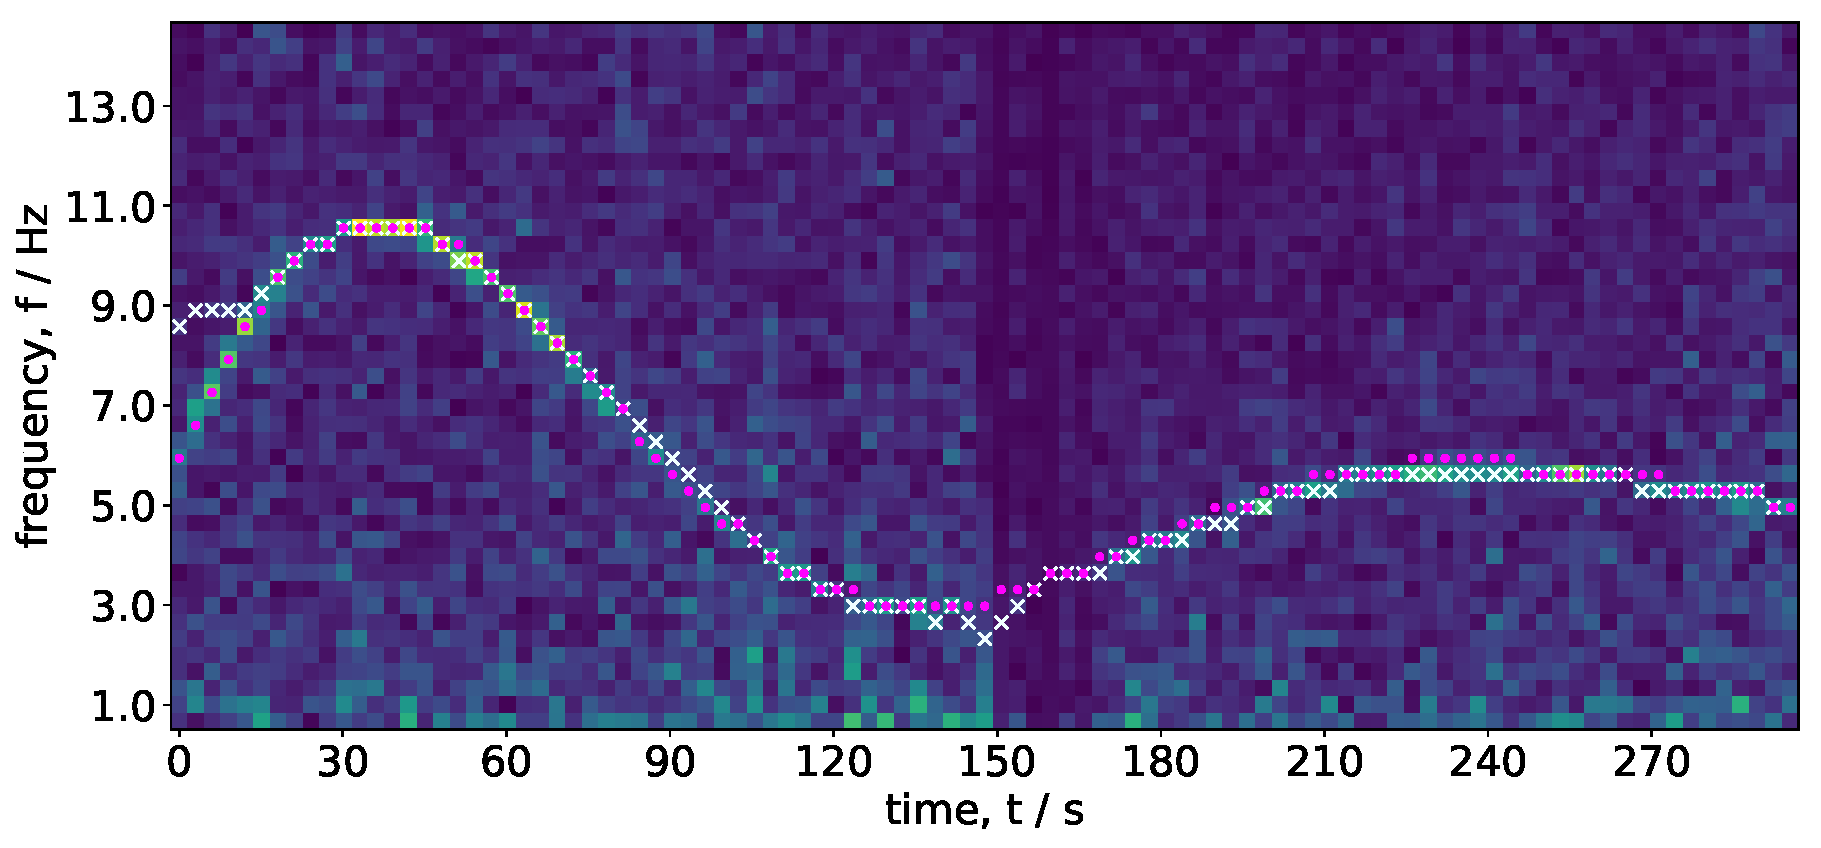
\includegraphics[width=\textwidth]{figures/expt_overlay_2_viterbi_test_webcam.pdf}
	\caption{\label{fig:viterbi_overlay}
Recovery of a wandering tone. 
The spectrogram shows the observed frequency amplitdue at each time-frequency step. 
The overlaid pink-dot and white-cross markers show the injected signal and recovered Viterbi path respetively. 
On the left, before $\sim 15\,{\rm s}$, the signal changes frequency too quickly for the Viterbi algorithm to recover. 
At $150\,{\rm s}$ the data appears anomalous, which may be due to some background noise. }
\end{figure*}


Our results are shown in Fig.~\ref{fig:viterbi_overlay}, where the heatmap shows the spectrogram of the observed signal. 
The overlaid pick-dot and white-cross markers show the injected signal and recovered Viterbi path respectively. 
The Viterbi path provides a good match to the injected frequency. 
%To the eye, the Viterbi algorithm easily recovers the injected frequency over time due to the high signal-to-noise ratio (SNR) of this experiment \han{What was the SNR? / can we quantify this?}.
Quantitatively, the Viterbi path is within one frequency bin ($\approx 0.3\,{\rm Hz}$) of the injected signal for $94\%$ of the time. 
%The Viterbi path stays within one frequency bin (approximately $0.3\,{\rm Hz}$) of the injected tone for $94\%$ of the run. 
Initially the injected signal moves faster then the frequency wander limit, leading to the discrepancy for $t\lesssim 10\,{\rm s}$. 
%Note that the signal initially moves faster than the frequency wander limit, causing a discrepancy between the injected and recovered signals. 
%To fix this, the limit should be doubled, although this would then cause the recovered path to stray more often. 
There is also an anomaly at $150\,{\rm s}$, which is likely due to a disturbance around the interferometer (such as someone walking nearby).
%There also appears to be an anomaly at $150\,{\rm s}$, likely from a disturbance (such as someone walking) around the interferometer.

%Empirically, decreasing the signal-to-noise ratio closer to unity (by making the speaker quieter) causes the Viterbi algorithm to stray more from the signal. 
%However, since the only correlation through the grid is the signal, we always expect the Viterbi path to lie near to the signal no matter how high the noise is, and this is indeed what we see. \han{Should we show results for this?}


\end{document}
